\documentclass[journal,onecolumn]{IEEEtran}
\usepackage[T1]{fontenc}
\usepackage{graphicx}
\begin{document}
\title{AirSense-R: Supplementary Error-Regime Diagnostics}
\author{Daniel~Oyewale\\
{\normalsize Ormedian Research Group}\\
{\normalsize\texttt{oyewaledanieloyewola@gmail.com}}}
\maketitle
\section{Descriptive concentration and seasonal comparisons}
Figure~\ref{fig:regimes} presents previously computed, accepted post-results
diagnostics from the leave-one-station-out evaluation. These comparisons use
equal-station averages of seed-level metrics; they do not pool all observations
as independent replicates. Every subgroup includes all 12 stations.
XGBoost has the lowest point MAE in the three bands below 200~$\mu$g/m$^3$;
persistence has the lowest point MAE in the highest band. This is a descriptive
comparison, not a claim of statistically established subgroup superiority.
The concentration bands describe observed targets and are not AQI categories.

\begin{figure}[!ht]
\centering
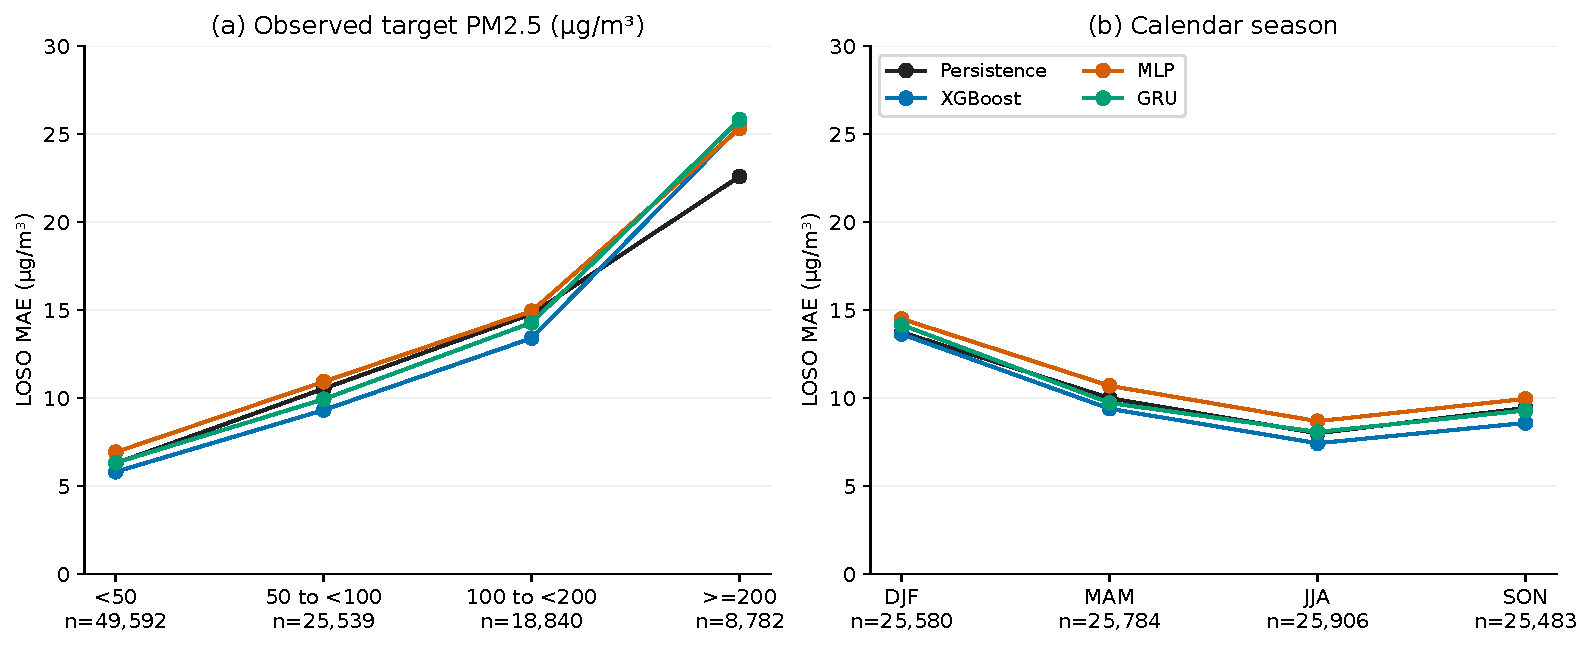
\includegraphics[width=\textwidth]{figures/descriptive_error_regimes.pdf}
\caption{Post-results descriptive error regimes. Points show MAE by observed
PM$_{2.5}$ band and calendar season; lines connect categories for readability.
No subgroup confidence intervals were computed. Counts denote distinct
station--target observations, not independent replications or per-model totals.
DJF: December--February; MAM: March--May; JJA: June--August; SON: September--November.
The full test year is March 2016--February 2017.}
\label{fig:regimes}
\end{figure}
\end{document}
